\chapter{Motivated work}
\label{chapter:motivated_work}
この章では, フローサイズの小さいトラフィックに対して,
MPTCPではTCPよりも通信性能が劣化すると報告された問題~\cite{improving}に対して,
大規模データセンターネットワークへのMPTCP適用時の問題点を把握するために, フローサイズの小さいトラフィックに対する性能を検証, 
ならびにクラウドサービスを想定したトラフィックの一例として並列分散処理アプリケーションを用いた二種類のトラフィックの測定結果を示す.
測定結果からトラフィックの特徴を示す事で, 従来のTCPで構成されたクラスターの抱えるボトルネックと複数のキュー,
複数の経路を持つマルチパス環境におけるデータセンターモデルの利点をそれぞれ示し, 提案手法の設計指針とする.

\section{再現実験のための予備実験}
\label{sec:reevaluation}
この節では, MPTCPデータセンターネットワークに対して実際のデータセンター環境を想定したシミュレーション実験として,
過去に行われた実験\cite{improving}の再現実験を行うために, 個々のデータセンタートラフィックに対するMPTCPとTCPの挙動の違いを検証する. 

\subsection{想定環境}
予備実験では, データセンターネットワーク上でpartition-aggregateモデルに従う並列分散処理を想定する.
ネットワークトポロジーについては, $k=4$ FatTreeトポロジーを用い,
全4ポッドの内, 1ポッド(4ノード)が管理ノード群として割り当てられ, 他ポッド(12ノード)に対して並列分散処理を割り当てる. 
またベンチマークトラフィックについては, \ref{sec:traffic}節で述べた内, 2つのトラフィックパターンについて評価・考察を行う.
メトリックとして表\ref{metric}を考える.

\begin{table}[t]
\begin{center}
\caption{Metric of each traffic patern}
\begin{tabular}{c|c}
\hline
トラフィックパターン & メトリック \\ \hline \hline
Query traffic & フロー完結時間[sec] \\
Short message traffic & フロー完結時間[sec] \\
Background traffic & スループット \\
\hline
\end{tabular}
%\ecaption{Metric of each traffic patern}
\label{metric}
\end{center}
\end{table}

\subsection{シミュレーション結果}

\subsubsection{Query traffic}
Query trafficに対する評価として, フローサイズを1KB$\sim$16KBとし, 
12の処理ノードへ平均200msのポアソン生起でトラフィックを発生させ, FCTを測定した.
また, Query trafficのみ発生させた場合と, 50\%の処理ノードに対し継続的にデータを送信するトラフィックであるBackground
trafficを同時に発生させた場合の2パターンについて評価を行った.
その結果を, Fig.\ref{fig:pure_query}, \ref{fig:mix_query}に示す.
なお, エラーバーとして99\%信頼区間を採用した.

この結果から, MPTCPはQuery trafficに対し, 直接性能に影響を及ぼさず, Background
Trafficによる影響が性能差を生じさせたことが分かる.
これは, 今のMPTCPの実装上, サイズの小さいデータ通信においては複数経路を利用せず, コネクション確立時に用いた経路のみで通信を完結するため,
Singlepath-TCPと同じ挙動となる. 
従って, Query trafficに対しては直接的にMPTCPが作用しない. 
一方で, サイズの大きいデータ通信に対しては複数の経路を利用し, 利用する経路分のスループットを達成できる. 
そのため, より多くのデータを転送し, 帯域を大きく占有するMPTCPの影響受け, Query trafficの遅延が生じたと考えられる. 

\begin{figure}[t]
    \begin{center}
    \includegraphics[autoebb, width=250pt]{./img/pure_query.pdf}
    \caption{Flow completion time of Query traffic with Background
    traffic}
    %\ecaption{Flow completion time  of Short message traffic with Background
    %traffic}
    \label{fig:pure_query}
    \end{center}
\end{figure}

\begin{figure}[t]
    \begin{center}
    \includegraphics[autoebb, width=250pt]{./img/mix_query.pdf}
    \caption{ Flow completion time  of Short message traffic with Background
    traffic}
    %\ecaption{Flow completion time  of Short message traffic with Background
    %traffic}
    \label{fig:mix_query}
    \end{center}
\end{figure}

\subsubsection{Short message traffic}
Short message trafficに対する評価として, フローサイズは50KB$\sim$1MBとした.
50\%の処理ノードに対し継続的にデータを送信するトラフィックを, Background trafficとして同時に発生させた状態で,
同時に12の処理ノードへ平均500msのポアソン生起でトラフィックを発生させ, FCTを測定した.
その結果を, Fig.\ref{fig:short_query}に示す.

この結果から, MPTCPはShort message trafficに対して直接的に作用し, FCTを短縮させたことが分かる.
これは, 先ほどのQuery trafficよりも大きいサイズのフローであるため, MPTCPにより複数経路を利用し,
TCPよりもより効率的な通信が行われたことを示している. 
実際フローサイズが小さいと, MPTCPによる恩恵も小さくなり, MPTCPとTCP間でFCTの差が小さくなっていることがわかる. 

\begin{figure}[t]
    \begin{center}
    \includegraphics[autoebb, width=250pt]{./img/mix_short.pdf}
    \caption{ Flow completion time  of Short message traffic with Background
    traffic}
    %\ecaption{Flow completion time  of Short message traffic with Background
    %traffic}
    \label{fig:short_query}
    \end{center}
\end{figure}

\section{再現シミュレーション}
\label{reproduction_simulation}
この節では,
Raiciuらによって示したFatTreeを用いたMPTCPネットワークモデルでのフローサイズの小さいトラフィックに対する性能評価シミュレーションを再現し,
解析を行った結果を示す.

\subsection{再現シミュレーション実験環境}
Raiciuらは~\cite{improving}において, 各プロトコルがフローサイズの小さなトラフィックに対して及ぼす影響の評価を行い,
フローサイズの小さいトラフィックに関しては, MPTCPによってFCTを遅延させることを示した.
そのときのシミュレーション環境は, 以下の通りである.
ネットワークトポロジーには, 4:1にオーバーサブスクリプションされたFatTreeを用いている.
ベンチマークトラフィックについては, エンドノード間の1対1通信を用いている.
全てのノード間通信のうち, 33\%をTCPまたはMPTCPにより継続してデータ転送 (バックグラウンドトラフィック)を行う.
残りのノードを使って, TCPによる70KBのデータ転送をを毎200msのポアソン生起させ, 転送完了までにかかった時間を計測している.

今回の再現実験にはns-3 Direct Code Execution~\cite{ns3}を用い, MPTCPは, Linux
カーネルソースを用いた~\cite{mptcp_linux}.
Fig.\ref{fig:fattree_rep}に, シミュレーションで用いたFatTree(k=2)トポロジーを示す.
このトポロジーでの物理パスでは, 一つのサブフローが1本の物理パスを占有するように, 設計している.
すなわち, 4つのサブフローを使う場合, ホストには4つのインターフェースに対しそれぞれ4つのIPアドレスが割り当てられることになる.
また, Host-Edge部分には, IPアドレスの数だけインターフェースを用意し, Aggregation-Edge部分も,
それに従いインターフェースを追加する.
さらにルーティングに関しては, インタフェースごとにCore1$\sim$Core4へと分散するようにルーティングテーブルを設定した.

表\ref{table:testbed}に再現シミュレーション環境に対する各パラメータをまとめる.
\begin{table}[t]
\begin{center}
\caption{Testbed on network simulation}
\begin{tabular}{c|c}
\hline
環境パラメータ & 値 \\ \hline \hline
ノード数 & 16 \\
MPTCP & v0.86 \\
帯域-core-aggr & 400Mbps \\
帯域-aggr-edge & 200Mbps \\
帯域-edge-host & 100Mbps \\
RTT & 0.5ms\\
バッファ & 100KB \\
\hline
\end{tabular}
%\ecaption{Testbed on network simulation}
\label{table:testbed}
\end{center}
\end{table}

\begin{figure}[t]
    \begin{center}
    \includegraphics[autoebb, width=250pt]{./img/fattree_rep.pdf}
    \caption{Network topology on reproducing simulation}
    %\ecaption{Network topology on reproducing simulation}
    \label{fig:fattree_rep}
    \end{center}
\end{figure}

\subsubsection{設定パラメータに対する有効性の検証}
伝搬遅延についてはRTT(Round Trip Time)として, 0.5msに設定した.
これは, 一般的なデータセンター内のRTTが1ms以下であるためである~\cite{rtt}.

ウィンドウサイズについては, 以下の帯域幅遅延積(BDP)の式から, 400Mbpsを最大限利用できるだけの値を設定した.
\begin{eqnarray}
BDP[{\rm byte}] = 帯域幅[{\rm bps}] \times RTT \div 8
\label{cong}
\end{eqnarray}

各帯域については, 16のノードを使って輻輳を引き起こす現象を再現するために, 実際のデータセンターのような広帯域のネットワークと比べ,
狭い帯域を設定した.

\subsection{再現結果}
Fig.\ref{fig:short_flow_rep}, Table.\ref{table:short_flow_rep}に,
上記の実験環境で再現した結果を示す.
再現結果から, フローの様子を完結時間別に4パターンに分類することができることが分かった.
表\ref{table:flow_pattern}にそのフローパターンの定義を示す.

\begin{figure}[t]
    \begin{center}
    \includegraphics[autoebb, width=250pt]{./img/flow_comp.pdf}
    \caption{The result of the reproduction experiment}
    \label{fig:short_flow_rep}
    \end{center}
\end{figure}

\begin{table}[t]
\begin{center}
\caption{Average flow completion time and stdev on reproduction experiment}
\begin{tabular}{c|c|c|c}
\hline
プロトコル & 平均フロー完結時間[ms] & 標準偏差[ms] & 95パーセンタイル[ms] \\ \hline \hline 
TCP & 78.4 & 122.5 & 266.7 \\
MPTCP & 91 & 140.6 & 510.5 \\
\hline
\end{tabular}
\label{table:short_flow_rep}
\end{center}
\end{table}

\begin{table}[t]
\begin{center}
\caption{Flow pattern classified by completion time}
\begin{tabular}{c|c|c}
\hline
フローパターン & 完結時間[ms] & パケットロスの有無 \\ \hline \hline
Full window & $\sim$30 & なし\\
Intensive flow & $\sim$60 & なし\\
Delay with loss & 200$\sim$300 & あり\\
Extreme delay & 300$\sim$ & あり\\
\hline
\end{tabular}
%\ecaption{Flow pattern classified by completion time}
\label{table:flow_pattern}
\end{center}
\end{table}


\subsection{考察}
Table.\ref{table:flow_pattern}に示した各フローパターンについて, それぞれの特性を分析する.

\subsubsection{パケットロスが発生しないフローパターン}
Fig.\ref{fig:full_intensive}にFull windowとIntensive flowのデータ転送の様子を示す.

Full windowではTCPコネクション確立後, サーバがすぐに最大ウィンドウサイズ分だけパケットを送り,
クライアントからのACKが返ってくると, 随時次のパケットを送っていた.
これは経路に輻輳がなく, 多くのウィンドウを利用できたということであり, 結果的に30ms以下でデータ転送を完了していた.

一方, Intensive flowでは, サーバが最大ウィンドウサイズ分に満たない量のパケットを送り,
クライアントからまとめて送られてくるACKを受け取った後, 集約してパケットを送っていた.
その結果, コネクションの切断時に, Full windowと比較して遅延を引き起こし60ms程度転送時間がかかった.

\subsubsection{パケットロスが生じたフローパターン}
Fig.\ref{fig:delay_loss}にDelay with lossとExtreme delayのデータ転送の様子を示す.
いずれのフローパターンもデータ転送中にパケットロスが発生し, 再送処理, 重複ACK確認応答を行った.
パケットロスが起きた原因は, 短時間にフローサイズの小さいトラフィックが中継ルータを集中したためである.
実際, 200msのポアソン生起のうち, 数10ms単位の短い期間でトラフィックが発生したとき, 中継ルータにおいてパケットロスが生じた.

Delay with lossでは, TCPコネクション確立後に数パケットのデータ転送を行い, パケットロスによるタイムアウトを生じた.
その後, 再送処理を経て, Maximum Segment Size (MSS)である1460byteでパケットを伝送した.

一方, Extreme delayでは, TCPコネクション確立直後にパケットロスによるタイムアウトを生じた.
その後も, パケットロスは生じないものの, 400ms頃まで遅延が生じていた.
また, Fig.\ref{fig:delay_loss}における二つのグラフの傾きは, セグメントサイズ最小値の586byteに設定され,
転送速度が上がらなかったことを表している.
これは, 中継するルータにおいてQoE制御による帯域制限が発生したことを示している.
実際, 同時刻に流れていたバックグラウンドトラフィックのスループットには変化がなく, QoE制御のrate
controlによりバックグラウンドトラフィックのデータ転送が優先され, ベンチマークトラフィックにはウィンドウサイズが制限されたと考えられる.

\begin{figure}[t]
    \begin{center}
    \includegraphics[autoebb, width=250pt]{./img/full_intensive.pdf}
    \caption{Comparison between Full window and Intensive flow}
    \label{fig:full_intensive}
    \end{center}
\end{figure}

\begin{figure}[t]
    \begin{center}
    \includegraphics[autoebb, width=250pt]{./img/flow_comp.pdf}
    \caption{Comparison between Delay with loss and Extreme delay}
    \label{fig:delay_loss}
    \end{center}
\end{figure}

\subsubsection{TCP v.s. MPTCP}
今回の再現実験において, TCPとMPTCPでFCTに差を生じた要因は, パケットロスが発生する割合にある.
Fig.\ref{fig:cdf}に再現実験でのFCTごとの累積確率分布を示す.
Fig.\ref{fig:cdf}からMPTCPでは, 遅延が生じたフローの割合が大きいことがわかる. 
これは, 前述の理由のようにMPTCPを用いることで, より多くの帯域が使われ, その結果一部のフローに対し,
パケットロスを生じるなどの遅延の影響があると考えられる. 
パケットロスを生じないフローに関しては, 遅延がなく両者に性能差を感じなかったが, MPTCPを用いた方が,
パケットロスを引き起こし遅延を生じさせる割合が大きいため, 全体的なサイズの小さい通信の性能としては劣化する. 

このようにMPTCPが帯域を大きく占有することにより他のトラフィックを圧迫することは, MPTCPの輻輳制御によるものだと考えられる.
混雑のない経路でデータ転送する場合, MPTCPでは積極的にウィンドウサイズを増やそうとするため, 他のフローに対し遅延を引き起こしたと推測される.


\begin{figure}[t]
    \begin{center}
    \includegraphics[autoebb, width=250pt]{./img/cdf_rep.pdf}
    \caption{CDF of flow completion time on reproduction experiment}
    %\ecaption{CDF of flow completion time on reproduction experiment}
    \label{fig:cdf}
    \end{center}
\end{figure}


\section{実トラフィック解析}

この節では, クラウドサービスを想定したトラフィックの一例として並列分散処理アプリケーションを用いた二種類のトラフィックの測定結果を示す.
測定結果からトラフィックの特徴を示す事で, \ref{reproduction_simulation}において考察した状況での遅延が起こる可能性の検証,
また従来のTCPで構成されたクラスターの抱えるボトルネックと複数のキュー, 複数の経路を持つマルチパス環境におけるデータセンターモデルの利点をそれぞれ示し, 提案手法の設計指針とする.

測定環境には, 管理ノード1台(Master), 処理ノード10台の計11台のクラスターPCを用いた.
管理ノードは10GbpsイーサネットリンクでTop of Rack(ToR)スイッチに接続されている.

このクラスターPCでPresto~\cite{presto}によりインタラクティブなレスポンスを返す, 分散SQLデータベースを実現しており,
$\S $\ref{sec:traffic}で示した三種類のトラフィックが混在している.
トラフィックの測定には, 管理ノードのインターフェースを用いて, tcpdump\cite{tcpdump}によるパケットレベルの測定を行った.

{\bf 定常状態: }
管理ノードに対し, ジョブ命令を一切与えていない中で約10時間程度トラフィックを測定した.
Fig.\ref{fig:constant}に定常時のフローサイズの累積分布を示す.
この分布から, 80\%以上のフローが10KB以下であるようにショートフローの数が全体のトラフィックの大部分を占めていることがわかる.
一方で通信量に着目すると, フロー数は比較的少ないがフローサイズの大きいトラフィックが大半を占めている.

次に, Fig.\ref{fig:constant_cdf}に管理ノードへのトラフィックの影響を示す.
この分布が示すように, 各処理ノードから管理ノードへのトラフィックの割合が大きく, それぞれフローサイズも大きい.
一方で, 管理ノードから各処理ノードへのトラフィックについては, 比較的フローサイズの小さいトラフィックの割合が大きい.
これは, Prestoの並列分散処理アーキテクチャ上,
YARNフレームワークなどにより各処理ノードの監視を担っている管理ノードから複数の処理ノードへフローサイズの小さいクエリーを送るという1対多通信と,
そのレスポンスとして, 複数の処理ノードから同時にノードの状態を送信するという, 多対1通信によるものである.

さらに, Fig.\ref{fig:constant_conc}に時間毎の同時接続数の分布を示す.
Fig.\ref{fig:constant_conc}中の長時間通信は通信時間が全測定時間の90\%以上であるフロー数を表している.
この分布が示すように, 各処理ノードから管理ノードへのトラフィックの同時接続数が多く, 積極的に通信が行われている.
また, 短い通信時間で通信が発生し終了する, スパイク性のあるトラフィックの中で長時間通信を行うフローが固定的に存在していることを示している. 

\begin{figure}[t]
    \begin{center}
    \includegraphics[autoebb, width=250pt]{./img/constant.pdf}
    \caption{Distribution of Presto cluster in a steady state}
    \label{fig:constant}
    \end{center}
\end{figure}

\begin{figure}[t]
    \begin{center}
    \includegraphics[autoebb, width=250pt]{./img/constant_cdf.pdf}
    \caption{CDF of the traffic from master node in a
    steady state}
    \label{fig:constant_cdf}
    \end{center}
\end{figure}

\begin{figure}[t]
    \begin{center}
    \includegraphics[autoebb, width=250pt]{./img/constant_conc.pdf}
    \caption{Distribution of the number of concurrent
    connections in a steady state}
    \label{fig:constant_conc}
    \end{center}
\end{figure}

{\bf 並列分散処理実行時: }
次に管理ノードに対し, 約1分間程度で完了するSQLジョブを与えた中でジョブが完遂するまでの間トラフィック測定を行った.
SQLジョブには, ``$select * from \, \$テーブル where \, \$条件$"を実行し,
全ての処理ノードにジョブを与えられるようにした.
Fig.\ref{fig:job}にジョブ実行時のフローサイズの累積分布を示す.
この分布が示すように, ショートフローの数が全体のトラフィックの大半を占めるが, 定常状態と比べると,
全体的にフローサイズ大きいトラフィックが増えている.
実際, 80\%以上のフローが110KB以下であるように, ショートフローの割合が小さくなった.
同様に通信量に着目すると, フロー数は比較的少ないがフローサイズの大きいトラフィックが大半を占めるという事が分かる.

次に, Fig.\ref{fig:job_cdf}に管理ノードへのトラフィックの影響を示す.
この分布が示すように, 各処理ノードから管理ノードへのトラフィックの割合が大きく, フローサイズは小さいものが多いことが分かる.
しかし, Fig.\ref{fig:constant_cdf}の定常時のトラフィックと比べると,
管理ノードから各処理ノードへのトラフィックの割合が大きくなっている.

さらに, Fig.\ref{fig:job_conc}に時間毎の同時接続数の分布を示す.
この分布が示すように, ジョブ実行中は全体的にフローの数は増え, とりわけ管理ノードから各処理ノードへのトラフィックの割合が大きくなっている.
さらに, ジョブ終了後も同時接続数が大きく変化していないことから, 長時間通信を行うフローが固定的に存在している.
また, 各処理ノードから管理ノードへのトラフィックに着目すると, ジョブ開始時に接続数が大きく増えている事から, バースト性があるトラフィックであるといえる.

\begin{figure}[t]
    \begin{center}
    \includegraphics[autoebb, width=250pt]{./img/job.pdf}
    \caption{Distribution of Presto cluster in executing a job}
    \label{fig:job}
    \end{center}
\end{figure}

\begin{figure}[t]
    \begin{center}
    \includegraphics[autoebb, width=250pt]{./img/job_cdf.pdf}
    \caption{CDF of the traffic from master node in executing a job}
    \label{fig:job_cdf}
    \end{center}
\end{figure}

\begin{figure}[t]
    \begin{center}
    \includegraphics[autoebb, width=250pt]{./img/job_conc.pdf}
    \caption{Distribution of the number of concurrent
    connections in executing a job}
    \label{fig:job_conc}
    \end{center}
\end{figure}

これらの分布から, クラウド型サービスを想定したトラフィックの特徴として以下の事が述べられる.
\begin{itemize}
  \item 定常時もジョブ実行時も同様に, 管理ノードへ送信されるトラフィック量は多い
  \item 長い時間通信を行うフローが固定的に存在している
  \item ジョブ実行時の処理ノードから管理ノードへのトラフィックには, フローサイズも小さく, バースト性がある
\end{itemize}

また, これらの特徴から, 管理ノードへのトラフィックの集中, ショートフローのバースト性,
そして長時間通信を行うBackgroung trafficの問題が生じていると考えられる.
従って, 管理ノードに対するトラフィックとして大きく二つのパターンを検討する必要がある.
\begin{enumerate}
  \item ジョブ開始時のバースト性のあるショートフロートラフィック
  \item アプリケーション性能に直接影響しないBackgroung trafficが通信している中で,
  低レイテンシ通信が求められているショートフローの通信
\end{enumerate}

こうしたトラフィックは主に, 複数の処理ノードから単一の管理ノードへの通信で発生する.
そして, 中継スイッチ, エンドノードともに単一のNICキューへとトラフィックが集中する事で, ボトルネックになり,
ショートフローの遅延が問題となる\cite{bottleneck}.

\subsection{性能障害}
\label{sec:expected_effect}
次に, これらのトラフィックパターンが引き起こす可能性のある二ヶ所のボトルネックについて検討する.

\subsubsection{スイッチ - 性能障害}
現在のスイッチ機器では複数のフローを多重に扱うための共有メモリを持ち, 共有メモリプールからMMU(Memory Management
Unit)によって各インターフェースが利用できるメモリ量を動的に割り当てる事で, 複数の通信を公平に処理する事を目指す~\cite{flexible}.
しかし, 比較的安価なスイッチでは制御できるメモリ量が制限されているため,
様々な性能障害を引き起こす~\cite{flexible}.

{\bf Incast}\\
\label{subsec:incast}
Fig.\ref{fig:impair}(a)に示すように, 短期間に一つのインターフェースへとフローが集中した場合, 用意されているキューが溢れ,
最悪の場合パケットロスを引き起こす.
こうしたトラフィックは, \S \ref{sec:traffic}で示したpartition-aggregate構造によるもので,
リクエストを受けた処理ノードが同期して一斉にレスポンスを返すことにより,
そのレスポンスを集約して受け取るノードが接続しているスイッチでのインターフェースのキューサイズが大きくなり, 遅延, パケットロスを生じる.
% こうした問題に対して, アプリケーションレベルにおいては二つのアプローチがある.
% 一つは, レスポンスのサイズを意図的に小さくし, スイッチバッファの圧迫を抑えることである.
% もう一つは, それぞれのリクエストにジッタを混ぜる事で, レスポンスを同期させないことである~\cite{synchro}.
% さらに, パケットロスを生じた際へのアプローチとしては, $RTO_{min}$を小さくする事でパケットロスの影響を抑える事ができる.

{\bf Queue buildup}\\
\label{subsec:queue}
\S \ref{sec:traffic}で示したように, 並列分散処理のレスポンスには直接影響しないBackgroung trafficは,
スイッチバッファにパケットロスを引き起こすほどの影響を及ぼし, そのインターフェースがボトルネックとなる可能性がある.
Fig.\ref{fig:impair}(b)に示すように, Backgroung trafficとQuery trafficが同じインターフェースを利用する場合に,
サイズの大きいフローによるショートフローのキューイング遅延が生じる.
このとき, Query trafficには{\it Incast}とは異なり, バースト性は必要ではない.
% このキューイング遅延の問題に対する解決策は, キューに溜まったパケットを素早く排出することで, キューサイズをなるべく小さく保つことである.

\begin{figure}[t]
    \begin{center}
    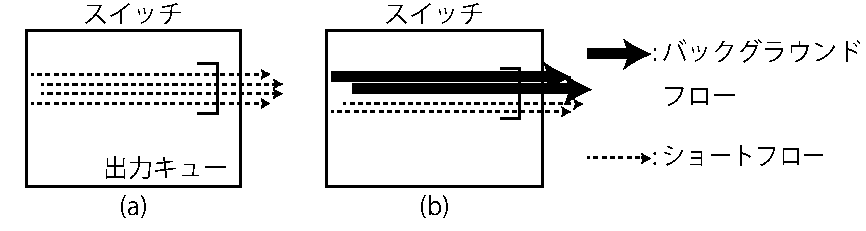
\includegraphics[autoebb, width=250pt]{./img/impairments.pdf}
    \caption{Bottoleneck in switch}
    \label{fig:impair}
    \end{center}
\end{figure}


\subsubsection{エンドノード - 性能障害}
今日のGbE(Gigabit Ethernet)通信において, 割込み処理は大きなボトルネック要因の一つである.
例えば, 1GbEにおいて64バイトフレームの最大受信可能数は, 毎秒約150万であり, 1パケット受信する度に割り込み処理を行うと,
CPUリソースが枯渇する.
そのため, 割込み処理の回数を抑えることが必要であるが, その分レイテンシが上がる可能性があり, 互いのトレードオフを適切に対処し高い性能を得る必要がある.
また, 今日の多くのCPUはマルチコアであり, CPUリソースを効率的に利用する事が求められている.

{\bf 割込み処理}\\
パケット受信の際のNICによるハードウェア割込みは, 即座に受信処理を行う事ができ, キューイングの遅延を小さくする事ができる.
しかし, 割込み処理が増えれば, その分オーバヘッドが大きくなり, OSの性能が劣化する.
割込み処理を扱う代表的な仕組みとして, ポーリング, interrupt coalescingがある.

ポーリングはNICの割り込みを使わず, タイマーにより定期的にNICの受信キューを監視することで, 割り込み負荷を軽減するソフトウェア技術である.
しかし, NICでパケットを受けてから即座に処理できない為, 遅延が発生する場合がある.
現在のLinuxカーネルにおいては, NAPIにより, 通信量が多く高負荷時にはポーリングが作用する~\cite{NAPI}

interrupt coalescingは, 複数のパケット, あるいは一定期間待ってからをまとめて一度で割り込ませる事で,
割込み回数を減らすハードウェア技術である.
しかし, ポーリングと同様, 即座に処理できない為, 遅延が発生する場合がある.

{\bf プロトコル処理}\\
マルチコア環境においても基本的には一つのNICの受信処理は1つのCPUでしか行えない.
そのため, ハードウェアへのアプローチとして, 1つのNICに複数の受信キューを持たせて, 受信処理をそれぞれのCPUへ分散させている, Receive
Side Scaling(RSS)がある~\cite{RSS}.
しかし, 一般に複数受信キューを持ち, RSS機能があるNICは高価である\cite{intel}.
そのため, 一つしか受信キューを持たないNICであっても, 複数のCPUを分散させるソフトウェア技術として, RPS(Receive Packet
Sterring)がある~\cite{RPS}.
しかしRPSでは, プロトコル処理とアプリケーション処理のCPUが異なる場合が生じ, その問題を最適化したのがRFS(Receive Flow
Sterring)がある~\cite{RFS}.
これらの技術により, CPUの複数のコアをより効率良く利用する事ができる.
また, プロトコル処理やアプリケーションでの処理については, RPS等で複数のCPUへと分散させる事ができるが,
その際の割込み処理についてはオーバヘッドが生じる可能性がある.


\section{検証実験}
\label{sec:verification}
% これまでの研究において報告されたMPTCPによるショートフロー性能劣化の問題~\cite{improving}を受け, その再現実験を行うことにより,
% 原因を解析し, 二つの要因を明らかにした~\cite{mptcp_ana}.
% 一つ目は, MPTCPはTCPよりも多くのトラフィックを排出し, より多くのNICインタフェースを利用する事で,
% 中継スイッチにおいてショートフローが利用するインタフェースと競合し, スイッチでの遅延, パケットロスが生じるということ.
% 二つ目は, ショートフロートラフィックのバースト性の問題により, エンドノードで単一のNICに負荷が集中し, 受信処理の遅延が生じたということ.
% これらの結果を受け,
% 低レイテンシでの通信が求められるショートフローに対して, MPTCPによるバックグラウンドトラフィックが利用しているインタフェースを回避し,
% 比較的輻輳が起こっていない経路を適切に選ぶ事で,
% 単一キューへの通信負荷の問題は解消され, ショートフローのフロー完結時間(FCT)が改善できるのではないかと, 仮説を立てた.
この節では, 実機での実験を用いて, 低レイテンシでの通信が求められるショートフローに対して,
バックグラウンドトラフィックが利用しているインタフェースを回避し, 適切に経路を選ぶ事で, 単一キューへの通信負荷の問題は解消され,
ショートフローのFCTが改善できるという仮説の検証, また複数のキュー,
複数の経路を利用した経路切り替えによる改善手法に対する予備実験を行う.
具体的には, 中継スイッチとエンドノードへのそれぞれの単一キューの負荷について, 複数のNICを用いて分散させ, その効果を検証する.

\subsection{実験環境}
{\bf (1)中継スイッチに対する負荷実験}\\
ネットワークトポロジーには, 2段で構成されたトポロジーを用いる.
Fig.\ref{fig:topology_switch}に, 用いたトポロジーを示す.
ベンチマークトラフィックについては, 二つのペアに対してエンドノード同士の1対1通信を用いている.
一方のペアに対しては, シミュレーションを実行している間, 継続してデータ転送 (バックグラウンドトラフィック)を行う.
他方のペアに対しては, TCPによる70Kbyteのデータ転送(ショートフロー)を毎10ms一様生起させ,
転送完了までにかかった時間FCT(Flow Completion Time)を計測する.
ショートフローのルーティングに関しては,
Fig.\ref{fig:topology_switch}に示す3つのパターンを用いて中継スイッチへのキューイング負荷の影響を検証する.


{\bf (2)エンドノードに対する負荷実験}\\
ネットワークトポロジーには, 二つのNICを持った二つエンドノード同士をL2スイッチを介してそれぞれのNIC毎に接続した.
Fig.\ref{fig:topology_node}に, 用いたトポロジーを示す.
ルーティングに関しては, それぞれの対をなすNIC同士が通信を行う.
ベンチマークトラフィックについては, エンドノード同士の1対1通信を用い, ショートフローとバックグラウンドフローを通信させる.
バックグラウンドフローについては,
ショートフローが通信しているNICペアと同じものを使って共有して通信させるパターンとショートフローが通信しているNICペアとは異なるペアのNICを用いて通信を行うパターンの2パターンについて検証する.
ショートフローは, TCPによる70Kbyteのデータ転送を毎10ms一様生起させ, 転送完了までにがかかった時間を計測している.
バックグラウンドトラフィックは, シミュレーションを実行している間, 継続してデータ転送を行う.

表\ref{table:experiment_ver}に用いた機器の詳細を示す.
\begin{figure}[t]
    \begin{center}
    \includegraphics[autoebb, width=250pt]{./img/topology_ns3.pdf}
    \caption{Topology in benchmark test for the NIC of
    the switch}
    \label{fig:topology_switch}
    \end{center}
\end{figure}

\begin{figure}[t]
    \begin{center}
    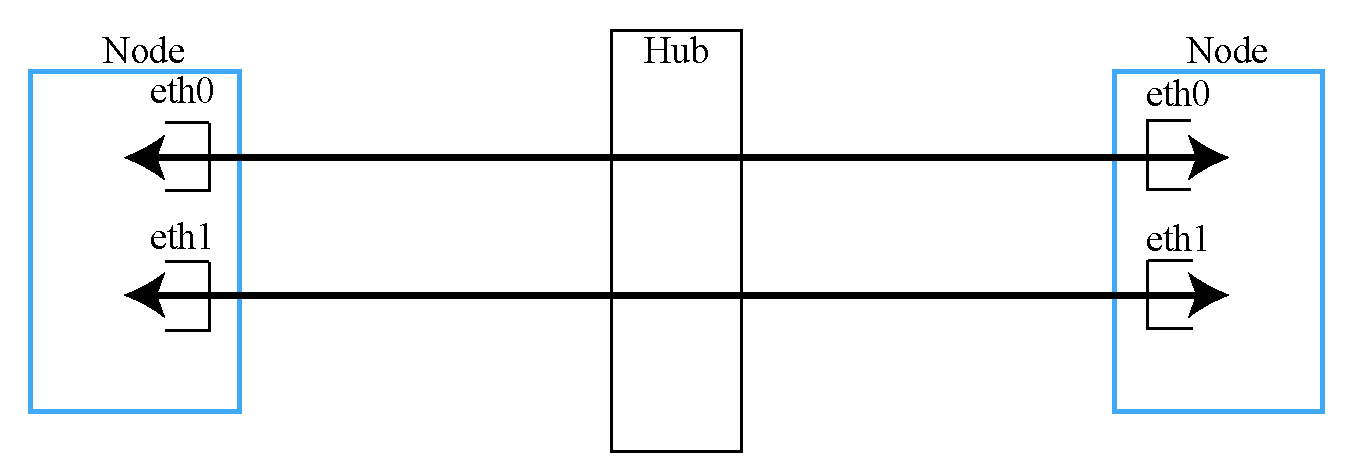
\includegraphics[autoebb, width=250pt]{./img/topology_real.pdf}
    \caption{ Topology in benchmark test for the NIC of
    the end-node}
    \label{fig:topology_node}
    \end{center}
\end{figure}

\begin{table}[t]
\begin{center}
\footnotesize
\begin{tabular}{c|c}
\hline
項目 & スペック \\ \hline \hline
OS & Linux 3.13.0 \\
CPU & Intel Xeon CPU L3426 \\
メモリー & 4GByte \\
NIC対応ドライバ & e1000 \\
スイッチ-実験1 & Catalyst 2940(100T) \\
スイッチ-実験2 & GS905L V2(1000T) \\
リンク & 1GbE \\
\hline
\end{tabular}
\caption{Experimental parameter}
\label{table:experiment_ver}
\end{center}
\end{table}

\subsection{実験結果}
{\bf (1)中継スイッチに対する負荷実験}\\
Fig.\ref{fig:improve}に上記の実験環境での結果として, 70KBのショートフローのFCTとバックグラウンドフローの経路利用率を示す.
FCTの箱ひげ図の上端には, 95パーセンタイル値, 下端には最小値を用いている.
最大値でなく95パーセンタイル値を採用したのは, 特に遅延した下位5パーセントに着目することで, 遅延した割合の大きさを比較するためである.
このメトリックにより, コンスタントにアプリケーション性能の出せるデータセンターネットワークの実現への指針となる.
この結果から, ショートフローの通信が中継スイッチにおいて, バックグラウンドフローと経路およびインターフェースを共有した影響で,
一部のフローが大きく遅延し, その分散が大きくなっている事が分かる.
一方で, 同じスイッチでインタフェースは共有しなかったフローに対しては大きな影響はなかった.
これは, 単一NICキューに対して二つのトラフィックが集中したことによる遅延の影響であると考えられる.
その影響からバックグラウンドフローに対しても, スループットが下がっている事が分かる.

これらの事から, アプリケーション性能に直接影響しないバックグラウンドフローが通信している中で,
低レイテンシ通信が求められているショートフローの通信をする際, 中継スイッチでの利用するインタフェースが競合する場合,
単一のキューに対しトラフィックが集中し, 受信処理の割込みのオーバヘッドや, プロトコル処理の遅延の影響が生じたと考えられる.

\begin{figure}[t]
    \begin{center}
    \includegraphics[autoebb, width=250pt]{./img/switch_verif.pdf}
    \caption{Link utilization and FCT of 70KB benchmark traffic for the switch}
    \label{fig:improve}
    \end{center}
\end{figure}


{\bf (2)エンドノードに対する負荷実験}\\
Fig.\ref{fig:real_exp0}に上記の実験環境での結果として,
70KBのショートフローのFCTとそれぞれの経路の利用率を示す.
FCTの箱ひげ図の上端には, 95パーセンタイル値, 下端には最小値を用いている.
この結果から, ショートフローの通信が, エンドノード間通信において, バックグラウンドフローと経路およびインターフェースを共有した影響で,
FCTの分散が大きくなっている事が分かる.
一方で, 経路, インタフェースは競合しなかったものの, バックグラウンドフローとショートフローが同時に通信を行ったことで若干の遅延の影響が生じ,
分散が大きくなっている.
これは, 単一NICに対して二つのトラフィックが集中したことによる負荷分散の効果が得られたが, プロトコル処理以降の部分で,
複数のフローが同時に通信を行った事に対するオーバヘッドが生じたと考えられる.
またバックグラウンドフローに着目すると, インターフェースを共有した場合においては,
ショートフローだけでなくバックグラウンドフローにも遅延が生じ, スループットが低下している.

これらの事から, アプリケーション性能に直接影響しないバックグラウンドフローが通信している中で,
バースト性のあるショートフロートラフィックの通信をする際, エンドノードに対して, 利用するインタフェースが競合する場合,
単一のNICに対しトラフィックが集中する事で, 受信処理の割込みのオーバヘッドや, プロトコル処理の遅延の影響があると考えられる.


\begin{figure}[t]
    \begin{center}
    \includegraphics[autoebb, width=250pt]{./img/real_eth0.pdf}
    \caption{Link utilization and FCT of 70KB benchmark traffic for the
    end-node}
    \label{fig:real_exp0}
    \end{center}
\end{figure}

\subsection{考察}
\label{sec:analysis}
これらの解析結果から, エンドノード, スイッチに対する機能障害が引き起こる要因について述べ, 今後の改善手法の検討を行う.
大量の計算機資源をいかに効率的に利用するか, という課題を今日のデータセンターは抱えており,
並列分散処理アプリケーションを用いる事が一般的である.
今の並列分散処理システムがpartition-aggrigation構造である限り, 管理ノードや多段のクラスター構成であればアグリゲーターノードに対して,
処理ノードからのトラフィックが集中する問題は発生する.
その結果, Queue buildupやIncastのような単一キューへの負荷集中の問題が中継スイッチやエンドノードに対して生じ,
CPU性能を効率的に引き出せず, 並列分散処理の性能が劣化する.

こうした遅延の影響を軽減する為には, 混雑時の通信量を抑える制御を行う, あるいは混雑時にも空いているリソースを効率良く利用する事が必要である.
MPTCPによる既存の計算機資源に対して複数NICを用いて性能向上を目指すように,
複数のフローを通信する際に異なる物理インターフェースを利用する事で, マルチコアを持つCPUの効率的な利用につなげられる.
すなわち, 複数のキューに対して通信を分散させるようなトラフィック制御により,
例えばレイテンシ志向なショートフローとスループット志向なバックグラウンドフローのような役割の異なるトラフィックを共存させ,
最適な通信の実現が可能であることが実験により明らかとなった.
そのような物理的に複数のNICによりマルチキューが介在する汎用的な機器で構成されているネットワークの中で,
トラフィックをどのように制御するかという点については, スイッチやエンドノードのOSスタック等のどこで制御をするか, またどのようなアルゴリズムでそれを実現するかを検討する必要がある.

\subsection{Directing result}
\label{sec:analysis}
経路混雑時のトラフィック制御について, 今後の指針となる一つの結果を示す.
提案手法では, 適切な経路を選んで通信を開始をする必要がある.
経路を決める際のメトリックとしては様々なものが考えられ, その中の一つとして経路の利用率がある.
経路利用率がショートフローの通信に対してどのような影響があるのか示した結果をFig.\ref{fig:load_test}に示す.
実験環境には, 中継スイッチに対する負荷実験と同様であり, バックグラウンドフローの負荷の度合いを変化させた.
この結果から, 70 $\sim$ 80 $ \% $ の経路利用率の場合, 遅延するショートフロー発生する事が分かり,
適切な経路選択には利用率も一要因として考慮する必要がある.

\begin{figure}[t]
    \begin{center}
    \includegraphics[autoebb, width=250pt]{./img/load_test.pdf}
    \caption{Impact of background flow for the switch}
    \label{fig:load_test}
    \end{center}
\end{figure}
